\section{Task 1}

\subsection{\textbf{Phân tích ngữ cảnh}}
\subsubsection{Mô tả chi tiết dự án}
\begin{center}
    \textbf{Hệ thống Quản lý Bãi đỗ xe Thông minh cho Khuôn viên Trường Đại học} 
\end{center}


$\noindent\hspace*{1cm}$ Trường Đại học Bách Khoa – Đại học Quốc gia TP. Hồ Chí Minh (HCMUT) mỗi ngày phải phục 
vụ một khối lượng lớn hoạt động gửi xe, bao gồm sinh viên đại học, học viên cao học, nghiên cứu sinh, 
giảng viên, cán bộ – nhân viên và khách vãng lai. Với mật độ phương tiện ngày càng tăng trong khi 
năng lực bãi đỗ xe có hạn, công tác quản lý hiện nay đang đối mặt với nhiều thách thức như ùn tắc tại 
các cổng ra vào, việc khai thác không hiệu quả các chỗ đậu xe, thiếu khả năng quan sát tình trạng chỗ 
trống theo thời gian thực, cũng như việc quản lý phí gửi xe còn phân tán và thiếu đồng bộ. Để giải 
quyết các vấn đề này, nhà trường có kế hoạch xây dựng một Hệ thống Quản lý Bãi đỗ xe Thông minh, 
ứng dụng các công nghệ Internet vạn vật (IoT) cùng với các nguyên lý hiện đại của công nghệ phần 
mềm. Hệ thống hướng tới việc hỗ trợ kiểm soát ra vào tự động, giám sát tình trạng bãi đỗ xe theo thời 
gian thực, điều hướng giao thông nội bộ một cách linh hoạt và tích hợp cơ chế tính phí – thanh toán, 
đồng thời phải hoạt động ổn định trong các điều kiện thực tế như số lượng người dùng lớn, kết nối 
không liên tục và sự đa dạng về nhóm người sử dụng. 

$\noindent\hspace*{1cm}$ Hệ thống được đề xuất phải hỗ trợ nhiều nhóm người dùng khác nhau, bao gồm người học 
(sinh viên, học viên cao học và nghiên cứu sinh), giảng viên, cán bộ – nhân viên và khách tạm thời. 
Các thành viên của trường sử dụng thẻ định danh chính thức để ra vào bãi xe, thẻ này được tích hợp 
với hạ tầng công nghệ của trường nhằm cho phép ghi nhận tự động các lượt vào và ra. Hoạt động gửi 
xe của người học được hệ thống tổng hợp theo một chu kỳ thanh toán xác định trước, sau đó hệ thống 
tự động tính toán phí tương ứng và khởi tạo yêu cầu thanh toán thông qua BKPay, nền tảng thanh toán 
nội bộ của nhà trường. Quyền lợi gửi xe và chính sách giá đối với giảng viên và cán bộ có thể khác 
nhau tùy theo quy định của từng thời kỳ và cần được cấu hình bởi các quản trị viên có thẩm quyền. 
Bên cạnh các người dùng đã được xác thực, hệ thống cũng phải hỗ trợ khách vãng lai và các trường 
hợp ngoại lệ, chẳng hạn như người dùng tạm thời không mang theo thẻ định danh. Trong những tình 
huống này, hệ thống cung cấp cơ chế truy cập tạm thời tại cổng vào, cho phép phát hành vé gửi xe và 
quản lý các phiên gửi xe độc lập với hệ thống xác thực tập trung. 

$\noindent\hspace*{1cm}$ Dưới góc độ IoT, hạ tầng bãi đỗ xe bao gồm nhiều chỗ đậu, trong đó mỗi chỗ được gắn với một cảm biến có nhiệm vụ phát hiện trạng thái có xe hoặc trống. Dữ liệu từ các cảm biến được thu thập 
và truyền về hệ thống trung tâm thông qua các cổng IoT cục bộ bằng các giao thức truyền thông tiêu 
chuẩn. Hệ thống cần duy trì được cái nhìn gần thời gian thực về tình trạng chỗ đậu xe, đồng thời có 
khả năng chịu lỗi trước các sự cố như cảm biến hỏng, mất kết nối gateway, hoặc dữ liệu bị trễ hay 
không nhất quán. Để cải thiện luồng giao thông và trải nghiệm người dùng trong khuôn viên trường, 
hệ thống phải hỗ trợ các cơ chế điều hướng tự động thông qua các bảng hiển thị điện tử được lắp đặt 
tại cổng bãi xe và các nút giao quan trọng. Các bảng này hiển thị động trạng thái bãi xe như còn chỗ, 
gần đầy hoặc hết chỗ, và có thể cung cấp thông tin chỉ dẫn tới các khu vực đỗ xe thay thế dựa trên dữ 
liệu thời gian thực của hệ thống. 
Hệ thống bãi đỗ xe thông minh phải được tích hợp với hạ tầng công nghệ hiện có của HCMUT. 
Việc xác thực đối với các thành viên trong trường được thực hiện thông qua HCMUT\_SSO, trong khi 
thông tin cá nhân và vai trò người dùng được đồng bộ từ HCMUT\_DATACORE theo cơ chế chỉ đọc 
nhằm đảm bảo tính nhất quán và an toàn dữ liệu. Cơ chế phân quyền dựa trên vai trò phải được áp 
dụng để hỗ trợ các trách nhiệm vận hành khác nhau, bao gồm người dùng cuối, nhân viên vận hành 
bãi xe và quản trị viên hệ thống. Tất cả các hoạt động gửi xe và giao dịch tài chính phải được ghi nhận 
đầy đủ để đảm bảo khả năng truy vết, phục vụ công tác kiểm tra, thống kê và báo cáo. 


\subsubsection{Mục tiêu dự án}
Để giải quyết các vấn đề trên, Hệ thống Quản lý Bãi đỗ xe Thông minh cho Khuôn viên Trường Đại học được đề xuất nhằm:
\begin{enumerate}
    \item Tự động hóa quy trình gửi xe
    \item Giảm thời gian chờ tại cổng
    \item Cung cấp thông tin thời gian thực về trạng thái bãi xe
    \item Đảm bảo tính chính xác trong tính phí
    \item Hỗ trợ thống kê và phân tích dữ liệu
\end{enumerate}

Hệ thống được tích hợp với các hệ thống bên ngoài như:

\begin{itemize}
    \item HCMUT\_SSO (xác thực người dùng nội bộ)
    \item HCMUT\_DataCore (đồng bộ dữ liệu người dùng)
    \item BKPay (xử lý thanh toán)
    \item IoT Gateway (cung cấp dữ liệu cảm biến chỗ đỗ)
\end{itemize}
Định hướng mở rộng trong tương lai

Trong tương lai, hệ thống có thể tích hợp AI để:
\begin{itemize}
    \item Nhận diện biển số tự động.
    \item Dự đoán tình trạng bãi xe.
    \item Áp dụng chính sách giá linh hoạt.
    \item Phát hiện bất thường trong vận hành.
\end{itemize}

\subsubsection{Các bên liên quan (stakeholder) \& lợi ích của các bên liên quan}


\ssssection{Người dùng nội bộ (Internal Users)}

Bao gồm sinh viên, giảng viên và cán bộ sử dụng bãi xe trong khuôn viên trường.

\textbf{Vai trò:}
\begin{itemize}
    \item Sử dụng bãi xe để gửi và lấy xe
    \item Thực hiện thanh toán phí gửi xe
    \item Kiểm tra tình trạng chỗ đỗ trước khi vào bãi
\end{itemize}

\textbf{Lợi ích:}
\begin{itemize}
    \item Quy trình ra/vào bãi xe nhanh chóng và thuận tiện
    \item Thanh toán phí gửi xe dễ dàng
    \item Có thông tin chính xác về số lượng chỗ đỗ còn trống
\end{itemize}

\ssssection{Khách vãng lai (Visitors)}

Bao gồm những người không thuộc hệ thống nội bộ nhưng có nhu cầu gửi xe trong thời gian ngắn.

\textbf{Vai trò:}
\begin{itemize}
    \item Sử dụng bãi xe trong thời gian ngắn
    \item Thanh toán phí gửi xe trực tiếp tại bãi
\end{itemize}

\textbf{Lợi ích:}
\begin{itemize}
    \item Quy trình sử dụng đơn giản và dễ tiếp cận
    \item Không yêu cầu đăng nhập hệ thống
    \item Thanh toán nhanh chóng và thuận tiện
\end{itemize}

\ssssection{ Nhân viên(Parking Operators)}

Là những người trực tiếp quản lý và vận hành bãi xe.

\textbf{Vai trò:}
\begin{itemize}
    \item Giám sát hoạt động của bãi xe
    \item Xử lý các sự cố phát sinh trong quá trình vận hành
    \item Hỗ trợ người dùng khi cần thiết
\end{itemize}

\textbf{Lợi ích:}
\begin{itemize}
    \item Hệ thống vận hành ổn định và đáng tin cậy
    \item Có giao diện giám sát trực quan để theo dõi tình trạng bãi xe
    \item Công cụ hỗ trợ xử lý sự cố nhanh chóng
\end{itemize}

\ssssection{ Quản trị viên (Administrators)}

Là những người chịu trách nhiệm quản lý và cấu hình hệ thống.

\textbf{Vai trò:}
\begin{itemize}
    \item Cấu hình chính sách giá và quyền lợi gửi xe
    \item Quản lý dữ liệu và hoạt động của hệ thống
    \item Theo dõi, tổng hợp và xuất báo cáo
\end{itemize}

\textbf{Lợi ích:}
\begin{itemize}
    \item Khả năng cấu hình hệ thống linh hoạt
    \item Dữ liệu thống kê chính xác và dễ truy xuất
    \item Đảm bảo tính bảo mật và an toàn của hệ thống
\end{itemize}

\ssssection{Hệ thống bên ngoài (External Systems)}

Các hệ thống tích hợp để hỗ trợ hoạt động của hệ thống bãi xe thông minh.

\textbf{Vai trò:}
\begin{itemize}
    \item \textbf{HCMUT\_SSO}: Xác thực danh tính người dùng nội bộ
    \item \textbf{HCMUT\_DataCore}: Đồng bộ và cung cấp thông tin người dùng
    \item \textbf{BKPay}: Xử lý các giao dịch thanh toán
    \item \textbf{IoT Gateway}: Cung cấp dữ liệu từ cảm biến về trạng thái chỗ đỗ
\end{itemize}

\textbf{Lợi ích:}
\begin{itemize}
    \item Tăng khả năng tích hợp và tự động hóa hệ thống
    \item Đảm bảo dữ liệu được đồng bộ và cập nhật liên tục
    \item Hỗ trợ vận hành hệ thống bãi xe hiệu quả và chính xác
\end{itemize}
\subsubsection{Phạm vi dự án}
\begin{enumerate}

\item \textbf{Quản lý người dùng và phân quyền:}
\begin{itemize}
    \item Xác thực người dùng nội bộ thông qua HCMUT\_SSO.
    \item Phân quyền truy cập theo vai trò: Người dùng nội bộ / Nhân viên / Quản trị viên.
    \item Quản lý thông tin người dùng và quyền lợi gửi xe.
\end{itemize}

\item \textbf{Quản lý hoạt động gửi xe:}
\begin{itemize}
    \item Hỗ trợ quẹt thẻ nội bộ khi vào/ra bãi xe.
    \item Hỗ trợ quẹt thẻ khách vãng lai.
    \item Tự động ghi nhận thời gian vào và ra.
    \item Kiểm tra và điều hướng trạng thái bãi xe theo thời gian thực.
\end{itemize}

\item \textbf{Quản lý thanh toán:}
\begin{itemize}
    \item Thanh toán tại chỗ đối với khách vãng lai.
    \item Thanh toán trả trước thông qua hệ thống tích hợp (BKPay).
    \item Tính phí tự động dựa trên chính sách giá hiện hành.
\end{itemize}

\item \textbf{Quản lý chính sách và vận hành hệ thống:}
\begin{itemize}
    \item Cấu hình chính sách giá và quyền lợi gửi xe.
    \item Giám sát và đồng bộ dữ liệu với hệ thống bên ngoài (HCMUT\_DataCore, IoT Gateway).
    \item Thống kê và xuất báo cáo doanh thu, lượt gửi xe.
    \item Xử lý sự cố tại chỗ và ghi nhận lịch sử thay dổi hệ thống.
\end{itemize}

\end{enumerate}
\newpage  
\subsection{\textbf{Phân tích yêu cầu}}

\subsubsection{Yêu Cầu Chức Năng}




\ssssection{\textbf{Yêu cầu chức năng phi tương tác}}
\begin{enumerate}
    \item [-] Hệ thống phải tự động điều chỉnh giá tiền phù hợp với thời gian thực (trước 18h là 2000đ, sau 18h là 3000đ).
    \item [-] Hệ thống phải tự động cập nhật trạng thái chỗ đậu xe dựa vào các cảm biến trong dưới 2 giây.
    \item [-] Hệ thống phải tự động ghi log và sao lưu lại dữ liệu mỗi 24h.
    \item [-] Hệ thống phải tự động phát hiện cảm biến không gửi dữ liệu trong không quá 5 phút.
    \item [-] Hệ thống phải tự động tạo báo cáo (Tỉ lệ đậu xe, số lượt sử dụng hàng ngày,...).
\end{enumerate}

\subsubsection{Yêu Cầu Phi Chức Năng}


\ssssection{\textbf{Hiệu năng (Performance)}}
\begin{enumerate}
    \item [-] Hệ thống phải xử lí yêu cầu của các phương tiện (vào/ra) trong không quá 2 giây.
    \item [-] Trạng thái bãi xe phải được cập nhật nhanh chóng và liên tục từ các cảm biến trong dưới 3 giây.
    \item [-] Hệ thống phải có khả năng hỗ trợ xử lý tối thiểu 300 người dùng đồng thời mà không làm giảm hiệu năng hệ thống.
\end{enumerate}
\ssssection{\textbf{Tính sẵn sàng và độ tin cậy (Availability \& Reliability)}}
\begin{enumerate}
    \item [-] Hệ thống phải luôn luôn hoạt động và ổn định 24/7, thời gian ngừng hoạt động phải không quá 1\%/tháng.
    \item [-] Hệ thống phải vẫn hoạt động ổn định khi có 1 hoặc nhiều cảm biến bị lỗi và thời gian phát hiện lỗi phải dưới 5 phút.
    \item [-] Tất cả dữ liệu ra/vào của phương tiện và thông tin người điều khiển phải được sao lưu tự động mỗi 30 phút.
\end{enumerate}
\ssssection{\textbf{Tính bảo mật (Security)}}
\begin{enumerate}
    \item [-] Người dùng phải đăng nhập thông qua hệ thống SSO của trường.
    \item [-] Tất cả thông tin đăng nhập và dữ liệu quan trọng phải được mã hóa bằng HTTPS/TLS.
    \item [-] Chỉ quản trị viên mới có quyền truy cập quyền quản trị hệ thống.
    \item [-] Tự động đăng xuất người dùng sau 30 phút không hoạt động.
\end{enumerate}
\ssssection{\textbf{Tính khả dụng và mở rộng (Scalability \& Maintainability)}}
\begin{enumerate}
    \item [-] Hệ thống phải hỗ trợ mở rộng tối thiểu 500 chỗ đậu xe cho bãi xe.
    \item [-] Hỗ trợ tích hợp thêm cảm biến mới mà không cần sửa toàn bộ hệ thống.
    \item [-] Mã nguồn phải được tổ chức rõ ràng, tuân thủ các chuẩn lập trình và có tài liệu hướng dẫn để thuận tiện cho việc bảo trì và xử lí các lỗi.
\end{enumerate}
\ssssection{\textbf{Tính thân thiện (Usability)}}
\begin{enumerate}
    \item [-] Giao diện phải trực quan, hiển thị đầy đủ trạng thái của bãi xe giúp cho người dùng dễ dàng xác định được chỗ trống trong dưới 30 giây.
    \item [-] Hỗ trợ đa ngôn ngữ (Tiếng Việt, Tiếng Anh, Tiếng Trung,...) để mở rộng tệp người dùng.
\end{enumerate}
\ssssection{\textbf{Tính tương thích (Compatibility)}}
\begin{enumerate}
    \item [-] Hệ thống có thể được truy cập trên nhiều trình duyệt web khác nhau (Chrome, FireFox,...) và trên thiết bị di động.
    \item [-] Hệ thống phải tương thích với hệ thống thanh toán BKPay với tỉ lệ gửi yêu cầu thanh toán thành công trên 99\%.
    \item [-] Hệ thống phải tích hợp được với hệ thống HCMUT SSO với tỉ lệ đăng nhập thành công trên 99\%.
    \item [-] Hệ thống phải hỗ trợ nhiều giao thức IoT tiêu chuẩn để kết nối với cảm biến và gateway.
\end{enumerate}
\ssssection{\textbf{Tính toàn vẹn dữ liệu (Data Integrity)}}
\begin{enumerate}
    \item [-] Mọi hoạt động của bãi xe (xe ra/vào, lịch sử thanh toán,...) phải được ghi log để thuận tiện cho việc kiểm tra.
    \item [-] Hệ thống phải có cơ chế backup dữ liệu ít nhất là 1 lần/ngày.
\end{enumerate}
\newpage  

\subsection{\textbf{Usecase diagram}}



\subsubsection{Cho toàn bộ hệ thống} 


    \begin{figure}[H]
        \centering
        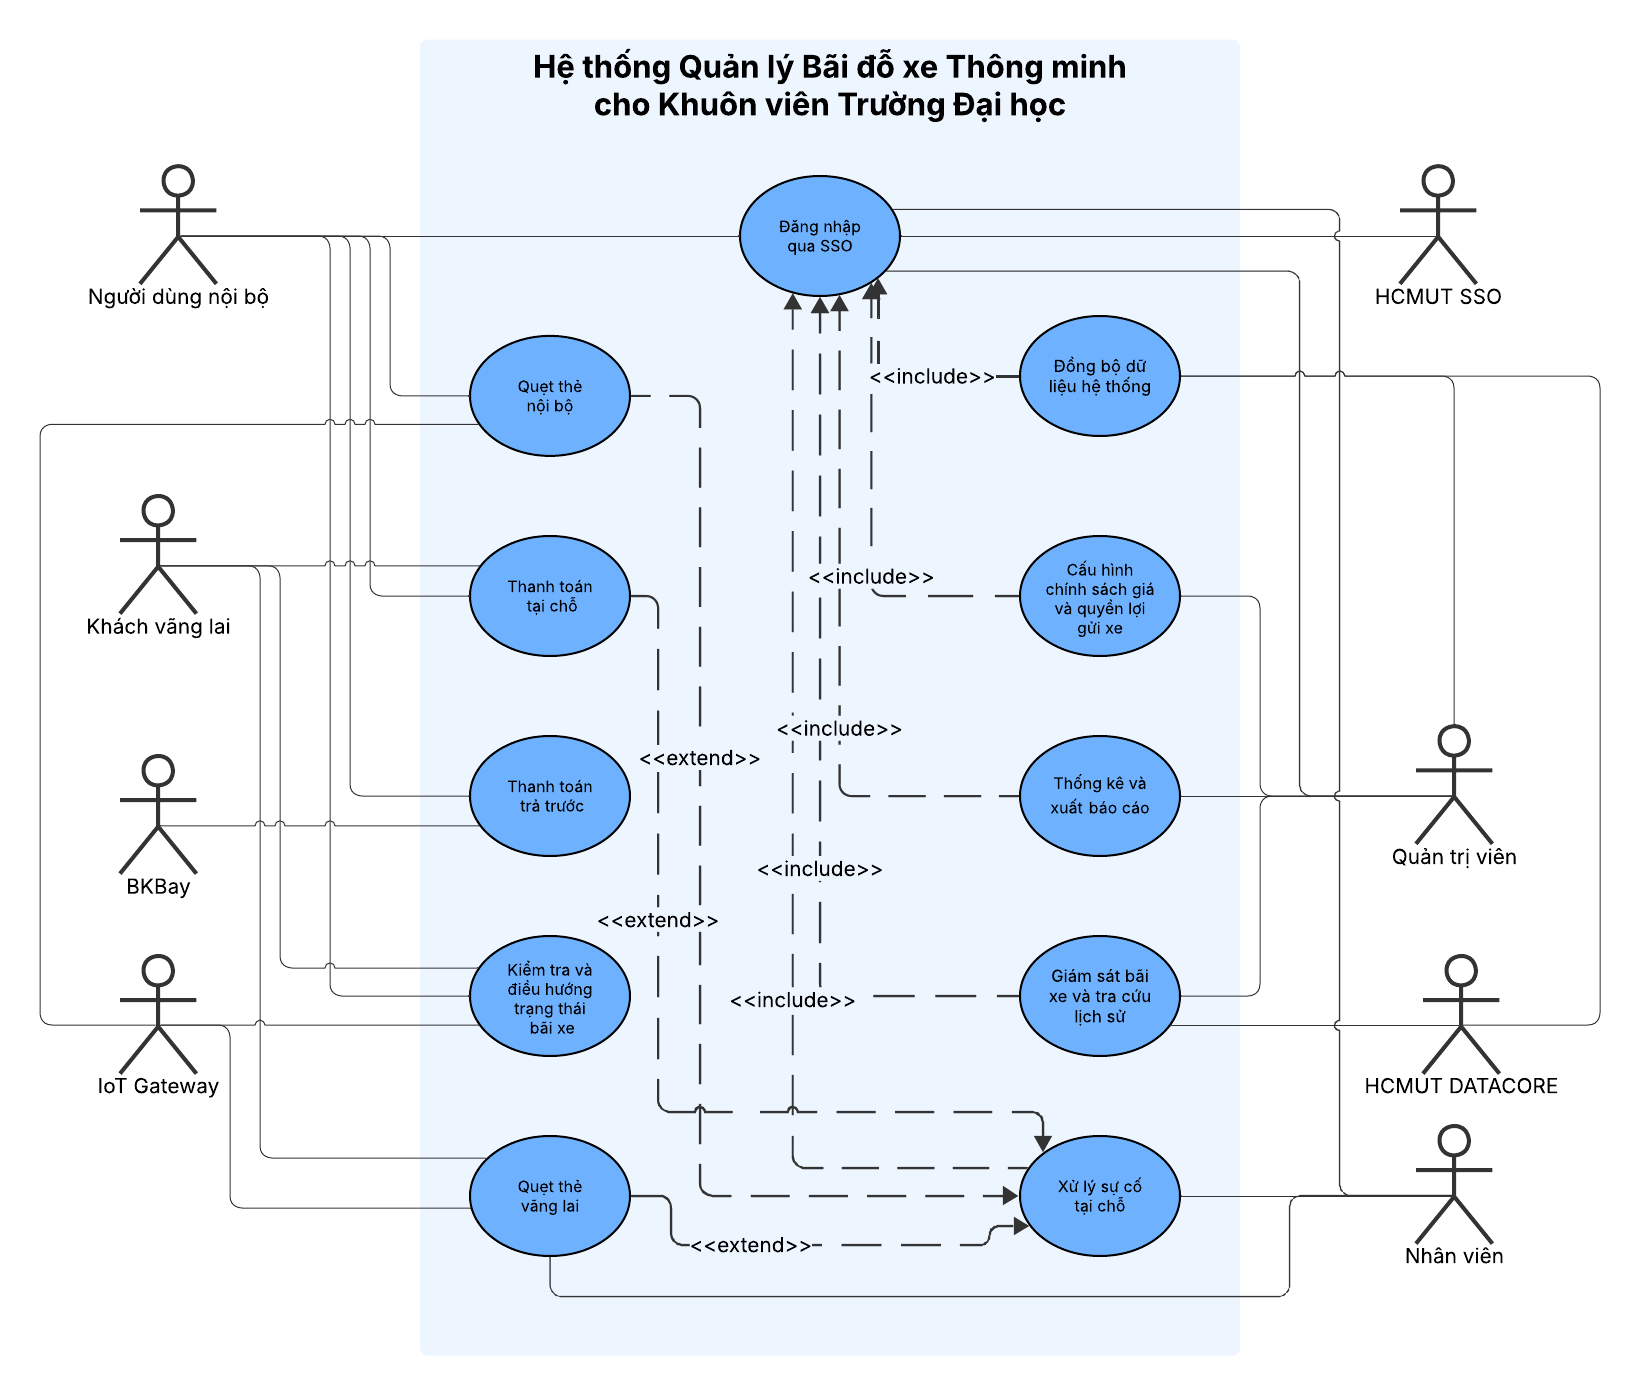
\includegraphics[scale=0.7]{Images/Task1/Use case diagram.png} 
        \caption{Use case diagram cho toàn bộ hệ thống}
    \end{figure}
    \bigskip

    Để giảm độ phức tạp khi đọc sơ đồ tổng quát, các use case trong hệ thống có thể được diễn giải theo các nhóm chức năng chính như sau:

    \begin{itemize}
        \item \textbf{Access Control}: bao gồm đăng nhập qua HCMUT SSO, quẹt thẻ nội bộ, quẹt thẻ vãng lai và các bước xác thực quyền ra/vào bãi xe.
        \item \textbf{Payment}: bao gồm thanh toán tại chỗ cho khách vãng lai và thanh toán trả trước hoặc thanh toán định kỳ thông qua BKPay.
        \item \textbf{IoT Monitoring and Guidance}: bao gồm cập nhật dữ liệu trạng thái từ IoT Gateway, hiển thị trạng thái bãi xe và điều hướng người dùng đến khu vực phù hợp.
        \item \textbf{Administration and Reporting}: bao gồm cấu hình chính sách giá, quyền lợi gửi xe, thống kê và xuất báo cáo.
        \item \textbf{Data Synchronization}: bao gồm đồng bộ thông tin định danh, vai trò người dùng và trạng thái liên quan từ các hệ thống ngoài như HCMUT\_DATACORE và BKPay về hệ thống nội bộ.
        \item \textbf{Incident Handling}: bao gồm ghi nhận, theo dõi và xử lý các sự cố tại chỗ như mất thẻ, lỗi camera, lỗi cổng hoặc lỗi thanh toán.
    \end{itemize}

    Trong đó, HCMUT\_DATACORE được xem là nguồn dữ liệu định danh và thông tin người dùng của trường. Các nghiệp vụ vận hành bãi xe như tạo phiên gửi xe, tính phí, đóng phiên, báo cáo và xử lý sự cố vẫn do hệ thống Smart Parking quản lý trong cơ sở dữ liệu nội bộ.


    \bigskip


\newpage

\subsubsection{Bảng mô tả usecase}

\textbf{Các use case cần mô tả: }
\vspace{-0.3cm}
\begin{center}
    \begin{tabular}{|c|l|m{7cm}|} \hline 
         \rule{0pt}{4ex}\textbf{Mã Usecase} & \textbf{Tên Usecase}& \textbf{Mô tả}\\[.2cm] \hline 
         \xrowht{30pt}   UC001   & Đăng nhập qua SSO                        & Nhân viên hoặc quản trị viên đăng nhập vào hệ thống thông qua HCMUT SSO để truy cập các chức năng quản lý. \\   \hline
         \xrowht{30pt}   UC002   & Quẹt thẻ nội bộ      & Người dùng nội bộ (sinh viên, giảng viên, cán bộ) quẹt thẻ định danh tại cổng để vào hoặc ra khỏi bãi xe. \\  \hline
         \xrowht{30pt}   UC003   & Quẹt thẻ vãng lai      & Khách vãng lai nhận vé hoặc quẹt thẻ tạm thời tại cổng để vào hoặc ra khỏi bãi xe. \\  \hline
         \xrowht{30pt}   UC004   & Thanh toán tại chỗ      & Khách vãng lai thực hiện thanh toán phí gửi xe trực tiếp tại cổng khi rời bãi xe.\\  \hline 
         \xrowht{30pt}   UC005   & Thanh toán trả trước   & Người dùng nội bộ thanh toán phí gửi xe định kỳ thông qua hệ thống BKPay. \\  \hline 
         \xrowht{30pt}   UC006A  & Cập nhật dữ liệu trạng thái bãi xe từ IoT Gateway & Hệ thống tiếp nhận, kiểm tra và cập nhật dữ liệu cảm biến từ IoT Gateway để duy trì trạng thái chỗ đỗ gần thời gian thực.\\  \hline
         \xrowht{30pt}   UC006B  & Hiển thị trạng thái bãi xe và điều hướng người dùng & Người dùng, nhân viên hoặc thiết bị hiển thị xem trạng thái bãi xe đã được cập nhật và nhận đề xuất khu vực đỗ phù hợp.\\  \hline 
        \xrowht{30pt}   UC007   & Cấu hình chính sách giá và quyền lợi gửi xe      & Quản trị viên thiết lập hoặc điều chỉnh chính sách giá và quyền lợi gửi xe cho từng nhóm người dùng. \\ \hline

          \xrowht{30pt}   UC008   & Thống kê và xuất báo cáo & Quản trị viên hoặc nhân viên xem và xuất báo cáo thống kê về lượt gửi xe, doanh thu và tình trạng bãi xe. \\  \hline 
         \xrowht{30pt}   UC009   & Giám sát bãi xe và tra cứu lịch sử & Hệ thống giám sát trạng thái các cảm biến, gateway để giám sát tình hình bãi xe và cho phép tra cứu lịch sử hoạt động của bãi xe. \\  \hline
         \xrowht{30pt}   UC010   & Đồng bộ dữ liệu hệ thống & Hệ thống tự động cập nhật thông tin người dùng và trạng thái tài chính từ hệ thống trường (SSO, DataCore, BKPay) ngay khi có xe ra/vào bãi. \\ \hline
         \xrowht{30pt}   UC011   & Xử lý sự cố tại chỗ & Nhân viên tiếp nhận phản ánh sự cố từ người dùng (ví dụ: mất thẻ, lỗi cổng, lỗi thanh toán), ghi nhận sự cố vào hệ thống và gửi thông báo đến quản trị viên để kiểm tra và xử lý. \\  \hline
    \end{tabular}
\end{center}

\newpage

\ssssection{Bảng mô tả usecase Đăng nhập qua SSO}


\begin{center}
    \begin{tabular}{|m{2.5cm}|m{13cm}|}
    \hline
        ID Use-case  & UC001 \\ 
        Name Use-case & Đăng nhập qua SSO \\ 
    \hline
        Actors & Người dùng nội bộ, Nhân viên, Quản trị viên, HCMUT\_SSO (Dịch vụ xác thực)\\
    \hline
        Description & Người dùng thực hiện đăng nhập vào hệ thống quản lý bãi đỗ xe thông minh thông qua dịch vụ xác thực HCMUT\_SSO. Sau khi xác thực thành công, hệ thống cho phép người dùng truy cập các chức năng tương ứng với vai trò của mình. \\
    \hline
        Trigger & Người dùng chọn nút “Đăng nhập qua SSO” trên giao diện hệ thống.\\
    \hline
        Preconditions & 
        1. Người dùng thuộc một trong các nhóm được phép truy cập hệ thống: người dùng nội bộ, nhân viên hoặc quản trị viên.
        
        2. Người dùng đã truy cập vào giao diện hệ thống quản lý bãi đỗ xe.
        
        3. Người dùng chưa đăng nhập vào hệ thống.
        
        4. Dịch vụ HCMUT\_SSO đang hoạt động bình thường.\\
    \hline
        Post conditions & 
        1. Người dùng được xác thực thành công bởi HCMUT\_SSO.
        
        2. Hệ thống tạo phiên đăng nhập cho người dùng.
        
        3. Người dùng được cấp quyền truy cập theo vai trò của mình (người dùng nội bộ, nhân viên hoặc quản trị viên).\\
    \hline
        Normal flow & 
        1. Người dùng chọn chức năng “Đăng nhập qua SSO”.
        
        2. Hệ thống chuyển hướng người dùng đến trang xác thực của HCMUT\_SSO.
        
        3. Người dùng nhập thông tin đăng nhập của tài khoản trường.
        
        4. HCMUT\_SSO kiểm tra tính hợp lệ của thông tin xác thực.
        
        5. Nếu xác thực thành công, HCMUT\_SSO trả kết quả xác thực về hệ thống.
        
        6. Hệ thống tạo phiên đăng nhập cho người dùng.
        
        7. Hệ thống chuyển người dùng đến giao diện chức năng phù hợp với vai trò của họ.\\
    \hline
        Alternative flow & 
        Ở bước 3, nếu người dùng chọn “Quên mật khẩu”, hệ thống chuyển người dùng sang chức năng khôi phục mật khẩu của HCMUT\_SSO.
        
        Ở bước 7, tùy theo vai trò người dùng:
        
        - Người dùng nội bộ được chuyển đến giao diện các chức năng cá nhân.
        
        - Nhân viên được chuyển đến giao diện vận hành bãi xe.
        
        - Quản trị viên được chuyển đến giao diện quản trị hệ thống.\\ 
    \hline
        Exception flow & 
        Ở bước 4, nếu thông tin đăng nhập không hợp lệ:
        
        - HCMUT\_SSO thông báo lỗi xác thực.
        
        - Người dùng được yêu cầu nhập lại thông tin đăng nhập.\\
    \hline
    \end{tabular}
\end{center}

\newpage

\ssssection{Bảng mô tả usecase Quẹt thẻ nội bộ}

\begin{center}
    \begin{longtable}{|>{\raggedright\arraybackslash}m{3.5cm}|m{12cm}|}
\hline
    \textbf{ID Use-case}  & UC002 \\ 
\hline
    \textbf{Name Use-case} & Quẹt thẻ nội bộ (Internal Card Check-in / Check-out) \\ 
\hline
    \textbf{Actors} & Người dùng nội bộ, Hệ thống IoT (IoT Gateway, Đầu đọc thẻ RFID, camera, Barrier), HCMUT\_DATACORE. \\
\hline
    \textbf{Description} & Hỗ trợ kiểm soát ra vào tự động bằng cách ghi nhận và xác thực thông tin xe của người dùng nội bộ (sinh viên, cán bộ) qua thẻ định danh đã được tích hợp thông tin người sử dụng trên hệ thống HCMUT\_DATACORE. \\
\hline
    \textbf{Trigger} & Người dùng nội bộ quẹt thẻ định danh của mình vào đầu đọc RFID tại trạm kiểm soát (cổng vào hoặc cổng ra). \\
\hline
    \textbf{Preconditions} & 
    1. Hệ thống trung tâm và các thiết bị phần cứng tại cổng (đầu đọc RFID, camera, barrier) đang hoạt động bình thường. \newline
    2. Thẻ định danh của người dùng đã được đồng bộ thông tin từ HCMUT\_DATACORE và đang ở trạng thái kích hoạt. \newline
    3. Đường truyền mạng giữa cổng IoT cục bộ và hệ thống trung tâm ổn định. \\
\hline
    \textbf{Post conditions} & Lượt ra/vào của người dùng được ghi nhận thành công; thanh chắn tự động đóng lại; trạng thái số chỗ trống của bãi xe được hệ thống cập nhật tự động (tăng/giảm) theo thời gian thực. \\
\hline
    \textbf{Normal flow} & 
    1. Đầu đọc thẻ RFID tại cổng IoT cục bộ nhận mã thẻ và truyền dữ liệu về hệ thống trung tâm. \newline
    2. Camera tại cổng đồng thời chụp lại hình ảnh biển số xe và người điều khiển. \newline
    3. Hệ thống đối chiếu mã thẻ với dữ liệu từ HCMUT\_DATACORE để xác thực quyền hạn ra vào của người dùng. \newline
    4. Nếu là lượt vào: Hệ thống khởi tạo một phiên gửi xe mới, liên kết mã thẻ với thời gian vào và biển số xe vừa nhận diện được. \newline
    5. Nếu là lượt ra: Hệ thống truy xuất phiên gửi xe hiện tại của thẻ, đối chiếu biển số xe chụp lúc ra với biển số xe đã lưu lúc vào. \newline
    6. Hệ thống gửi lệnh qua IoT Gateway để mở thanh chắn (barrier) cho phương tiện di chuyển. \newline
    7. Sau khi xe đi qua, hệ thống ghi nhận đầy đủ giao dịch vào cơ sở dữ liệu để phục vụ truy vết và báo cáo. \\
\hline
    \textbf{Exception flow} & 
    1. \textbf{Thẻ không hợp lệ / không có quyền trên HCMUT\_DATACORE}: Hệ thống hiển thị thông báo từ chối trên màn hình LED tại cổng, phát âm thanh cảnh báo và barrier không mở. \newline
    2. \textbf{Không nhận diện được biển số (camera lóa, khuất)}: Hệ thống cảnh báo lỗi đọc camera. Hệ thống báo động để nhân viên xử lý sự cố tại chỗ (UC10) kiểm tra hình ảnh thực tế và nhập biển số thủ công vào hệ thống để tiếp tục quy trình. \newline
    3. \textbf{Biển số ra không khớp biển số vào}: Barrier không mở. Hệ thống báo động để nhân viên xử lý sự cố tại chỗ (UC10) ra đối chiếu giấy tờ xe thủ công. \newline
    4. \textbf{Mất kết nối mạng}: Cổng IoT chuyển sang chế độ offline, cho phép mở barrier dựa trên danh sách thẻ hợp lệ (whitelist) đã được lưu sẵn cục bộ tại cổng và lưu trữ dữ liệu lượt vào/ra để tự động đồng bộ lên hệ thống trung tâm khi có mạng trở lại. \\
\hline
\end{longtable}
\end{center}

\newpage

\ssssection{Bảng mô tả usecase Quẹt thẻ vãng lai }


\begin{center}
    \begin{longtable}{|>{\raggedright\arraybackslash}m{3.5cm}|m{12cm}|}
\hline
    \textbf{ID Use-case}  & UC003 \\ 
\hline
    \textbf{Name Use-case} & Quẹt thẻ vãng lai (Visitor Card Check-in). \\ 
\hline
    \textbf{Actors} & Nhân viên vận hành bãi xe, Khách vãng lai, Hệ thống IoT (Đầu đọc thẻ RFID, Camera, Barrier). \\
\hline
    \textbf{Description} & Nhân viên bãi xe sử dụng thẻ vãng lai (thẻ RFID dùng chung của bãi) để phát cho khách lúc vào, ghi nhận hình ảnh/biển số xe. Khi khách ra, nhân viên thu lại thẻ, hệ thống đối chiếu biển số để nhân viên thu tiền trực tiếp. Quá trình này tạo ra một phiên đỗ xe tạm thời, không yêu cầu thiết lập tài khoản cá nhân. \\
\hline
    \textbf{Trigger} & 
    - Lượt vào: Nhân viên quẹt một thẻ vãng lai trống vào đầu đọc để phát cho khách. \newline
    - Lượt ra: Nhân viên nhận lại thẻ từ khách và quẹt vào đầu đọc để kiểm tra. \\
\hline
    \textbf{Preconditions} & 
    1. Hệ thống hoạt động bình thường. \newline
    2. Nhân viên trực cổng có sẵn danh sách thẻ vãng lai trống (chưa gắn với xe nào đang trong bãi). \\
\hline
    \textbf{Post conditions} & Phiên đỗ xe của khách vãng lai hoàn tất và được lưu lại lịch sử (giờ vào/ra, ảnh, biển số) vào CSDL để phục vụ truy vết. Thẻ vãng lai được thu hồi để tái sử dụng. Nhân viên đã thu được tiền mặt. \\
\hline
    \textbf{Normal flow} & 
    \textbf{Luồng vào (Check-in):} \newline
    1. Nhân viên quẹt thẻ vãng lai vào đầu đọc. \newline
    2. Camera tự động chụp biển số và hình ảnh người lái xe. \newline
    3. Hệ thống tạo một "phiên đỗ xe tạm", gắn mã thẻ với hình ảnh/biển số vừa chụp và lưu giờ vào. (Không lưu thông tin định danh nào khác). \newline
    4. Nhân viên đưa thẻ cho khách vãng lai và khách lái xe vào bãi sau đó hệ thống mở barrier. \newline
    \newline
    \textbf{Luồng ra (Check-out):} \newline
    5. Khách ra cổng và trả lại thẻ cho nhân viên. \newline
    6. Nhân viên quẹt thẻ vào đầu đọc. \newline
    7. Camera chụp hình ảnh/biển số lúc ra. \newline
    8. Hệ thống hiển thị hình ảnh/biển số lúc vào và lúc ra lên màn hình của nhân viên để đối chiếu, đồng thời tính toán phí gửi xe dựa trên thời gian đỗ. \newline
    9. Nhân viên thu tiền mặt trực tiếp từ khách và bấm xác nhận hoàn tất trên phần mềm. \newline
    10. Hệ thống kết thúc "phiên đỗ xe tạm", reset thẻ về trạng thái trống và mở barrier cho khách ra. \\
\hline
    \textbf{Exception flow} & 
    1. \textbf{Biển số ra không khớp biển số vào}: Hệ thống cảnh báo đỏ trên màn hình, barrier không mở. Nhân viên yêu cầu khách xuất trình giấy tờ xe để xử lý thủ công (kích hoạt UC10: Xử lý sự cố tại chỗ). \newline
    2. \textbf{Khách làm mất thẻ (Lượt ra)}: Nhân viên yêu cầu khách cung cấp biển số xe, nhân viên tìm kiếm thủ công trên phần mềm để lấy thông tin lượt vào. Hệ thống tính phí đỗ xe + phí phạt mất thẻ. Nhân viên thu tiền, bấm mở barrier thủ công và hệ thống đánh dấu thẻ bị mất là "Đã khóa". \newline
    3. \textbf{Camera không đọc được biển số}: Nhân viên chủ động gõ biển số bằng tay vào phần mềm hệ thống để điền khuyết dữ liệu rồi mới cho xe qua. \\
\hline
\end{longtable}
\end{center}

 

\newpage

\ssssection{Bảng mô tả usecase Thanh toán tại chỗ}

\begin{center}
    \begin{tabular}{|m{2.5cm}|m{13cm}|}
    \hline
        ID Use-case  & UC004 \\ 
        Name Use-case & Thanh toán tại chỗ \\ 
    \hline
        Actors & Người dùng nội bộ, khách vãng lai, nhân viên, \\
    \hline
        Description & gười dùng thanh toán phí gửi xe trực tiếp tại bãi xe khi rời bãi. Hệ thống tính phí dựa trên thông tin phiên gửi xe và chính sách giá hiện hành.\\
    \hline
        Trigger & Người dùng quẹt thẻ tại cổng ra của bãi xe.\\
    \hline
        Preconditions & 
        1. Người dùng đã có một phiên gửi xe hợp lệ trong hệ thống.
        
        2. Thông tin phiên gửi xe đã được ghi nhận khi vào bãi.

        3. Hệ thống có thể truy xuất dữ liệu phiên gửi xe.
        
        4. Dịch vụ HCMUT\_SSO đang hoạt động bình thường.\\
    \hline
        Post conditions & 
        1. Phí gửi xe được thanh toán thành công.
        
        2. Phiên gửi xe được đóng trong hệ thống.
        
        3. Cổng ra được mở cho phép người dùng rời bãi xe.
        
        4. Thông tin giao dịch được lưu vào hệ thống để phục vụ thống kê và báo cáo.\\
    \hline
        Normal flow & 
        1. Người dùng quẹt thẻ tại cổng ra của bãi xe.
        
        2. Hệ thống xác định phiên gửi xe tương ứng với thẻ.
        
        3. Hệ thống tính phí gửi xe dựa trên:

            - Thời điểm vào bãi

            - Thời điểm ra bãi

            - hính sách giá hiện hành.
        
        4. Hệ thống hiển thị số tiền cần thanh toán.
        
        5. Người dùng thực hiện thanh toán tiền  tại chỗ.
        
        6. Nhân viên bãi xe xác nhận thanh toán trong hệ thống.
        
        7. Hệ thống đóng phiên gửi xe.
        
        8. Cổng ra được mở để người dùng rời bãi.\\
    \hline
        Alternative flow & 
       \textbf{Alternative 1:} Người dùng nội bộ có gói trả trước.

        1. Hệ thống phát hiện người dùng có gói gửi xe trả trước còn hiệu lực.

        2. Hệ thống không yêu cầu thanh toán.

        3. Phiên gửi xe được đóng.

        4. Cổng ra được mở.

         \textbf{Alternative 2:} Thanh toán bằng phương thức điện tử tại quầy.

        1. Người dùng chọn thanh toán bằng QR.

        2. Hệ thống xác nhận giao dịch thành công.

        3. Hệ thống cập nhật trạng thái thanh toán.

        4. Cổng ra được mở. 
        \\ 
    \hline
    \end{tabular}
\end{center}
\begin{center}
    \begin{tabular}{|m{2.5cm}|m{13cm}|}
    \hline
        Exception flow & 
        \textbf{Exception 1:} Không tìm thấy phiên gửi xe.

        1. Hệ thống không tìm thấy phiên gửi xe tương ứng với thẻ.

        2. Hệ thống thông báo lỗi cho nhân viên bãi xe.

        3. Nhân viên thực hiện xử lý sự cố tại chỗ.
    
        \\
    \hline
    \end{tabular}
\end{center}

\newpage

\ssssection{Bảng mô tả usecase Thanh toán trả trước}


\begin{center}
    \begin{tabular}{|m{2.5cm}|m{13cm}|}
    \hline
        ID Use-case  & UC005 \\ 
        Name Use-case & Thanh toán trả trước \\ 
    \hline
        Actors & Người dùng nội bộ, BKPay, HCMUT DataCore\\
    \hline
        Description & Tính năng cho phép người dùng nội bộ đăng ký hoặc gia hạn gói gửi xe trả trước theo chu kỳ. Sau đó thực hiện thanh toán thông qua BKPay, hệ thống xác thực và kích hoạt gói gửi xe cho tài khoản người dùng. \\
    \hline
        Trigger & Người dùng chọn "Gửi xe trả trước" trên hệ thống.\\
    \hline
        Preconditions & 
        1. Người dùng đã đăng nhập hệ thống thành công thông qua HCMUT SSO.

        2. Người dùng có thẻ id nội bộ (thẻ sinh viên, ...)
        
        3. Hệ thống BKPay đang hoạt động.
        \\
    \hline
        Post conditions & 
        1. Gói gửi xe trả trước được kích hoạt hoặc gia hạn cho người dùng.
        
        2. Thông tin thanh toán được lưu vào hệ thống.
        
        3. Người dùng có thể sử dụng thẻ nội bộ để gửi xe trong thời gian gói còn hiệu lực.\\
    \hline
        Normal flow & 
        1. Người dùng chọn chức năng "Gửi xe trả trước".
        
        2. Hệ thống hiển thị danh sách các gói gửi xe trả trước (ví dụ: gói tuần, gói tháng, gói học kỳ, ...).
        
        3. Người dùng chọn một gói gửi xe phù hợp.
        
        4. Hệ thống hiển thị thông tin chi tiết của gói(thời hạn, giá tiền, quyền lợi) và tùy chọn "Đăng ký" hoặc "Gia hạn".
        
        5. Người dùng chọn "Đăng ký" và hệ thống hiện tùy chọn "Xác nhận" hoặc "Hủy".
        
        6. Sau khi người dùng chọn xác nhận, hệ thống gửi yêu cầu thanh toán đến BKPay.
        
        7. BKPay hiển thị giao diện thanh toán cho người dùng.
        
        8. Người dùng thực hiện thanh toán trên BKPay.
        
        9. BKPay gửi kết quả thanh toán về hệ thống.
        
        10. Hệ thống xác thực thành công và kích hoạt gói gửi xe cho tài khoản người dùng.
        
        11. Hệ thống thông báo thanh toán thành công.\\
        \hline
    \end{tabular}
\end{center}

\begin{center}
    \begin{tabular}{|m{2.5cm}|m{13cm}|}
    \hline
        Alternative flow & 
        \textbf{Alternative 1:} Gia hạn khi gói hiện tại vẫn còn hiệu lực.
        
        1. Người dùng chọn gói bất kỳ và nhấn "Gia hạn".

        2. Hệ thống hỏi người dùng có muốn gia hạn bằng gói này hay không và người dùng chọn "Xác nhận".
        
        3. Sau khi thanh toán thành công, hệ thống cộng thêm thời gian gói mới vào thời hạn hiện tại. 
        
         \textbf{Alternative 2:} Người dùng đăng ký 1 gói khác khi gói hiện tại đang còn hiệu lực.
        
        1. Người dùng chọn 1 gói và ấn "Đăng ký".

        2. Hệ thống gửi thông báo lên màn hình "Gói hiện tại vẫn đang còn hiệu lực, hãy gia hạn !" khoảng 3 giây thì biến mất.

        3. Người dùng chọn "Gia hạn" hoặc thoát khỏi hệ thống.

         \textbf{Alternative 3:} Người dùng hủy giao dịch thanh toán.
        
        1. Trong bước thanh toán, người dùng chọn hủy giao dịch trên BKPay.

        2. BKPay gửi trạng thái hủy về hệ thống.

        3. Hệ thống hủy yêu cầu thanh toán và hiện thông báo thanh toán thất bại.
        \\ 
    \hline
        Exception flow & 
        \textbf{Exception 1:} Thanh toán thất bại.
        
        1. BKPay không thể xử lý giao dịch thanh toán(có thể do ứng dụng ngân hàng bị lỗi, tình trạng kết nối mạng hoặc do hệ thống BKPay).

        2. BKPay gửi trạng thái thất bại về hệ thống.

        3. Hệ thống hiển thị thông báo thanh toán thất bại cho người dùng.

        \textbf{Exception 2:} Không kết nối được BKPay.
        
        1. Hệ thống không thể gửi yêu cầu thanh toán đến BKPay.

        2. Hệ thống thông báo lỗi và yêu cầu người dùng thử lại sau.\\
        \hline
    \end{tabular}
\end{center}

 

\newpage

\ssssection{Bảng mô tả usecase Cập nhật dữ liệu trạng thái bãi xe từ IoT Gateway}

\begin{center}
\begin{longtable}{|m{2.7cm}|m{12.8cm}|}
\hline
ID Use-case  & UC006A \\ 
Name Use-case & Cập nhật dữ liệu trạng thái bãi xe từ IoT Gateway \\ 
\hline
Actors & Primary actor: IoT Gateway. Supporting actors: Hệ thống Smart Parking, Dịch vụ cảnh báo, Nhân viên vận hành.\\
\hline
Description & Use case này mô tả phần hệ thống tiếp nhận, kiểm tra và cập nhật dữ liệu cảm biến từ IoT Gateway. Mục tiêu là duy trì dữ liệu trạng thái chỗ đỗ gần thời gian thực trước khi dữ liệu này được dùng cho màn hình hiển thị hoặc chức năng điều hướng ở UC006B.\\
\hline
Trigger & IoT Gateway gửi gói dữ liệu mới về trạng thái các cảm biến chỗ đỗ, hoặc hệ thống nhận lịch đồng bộ định kỳ từ gateway.\\
\hline
Preconditions & 
1. Hệ thống Smart Parking đang hoạt động.

2. Danh sách khu vực, chỗ đỗ và mã cảm biến đã được cấu hình.

3. IoT Gateway có thể gửi dữ liệu qua kênh kết nối đã đăng ký, hoặc hệ thống còn dữ liệu gần nhất để dùng tạm thời.\\
\hline
Post conditions & 
1. Trạng thái chỗ đỗ và khu vực được cập nhật trong cơ sở dữ liệu nội bộ nếu dữ liệu hợp lệ.

2. Hệ thống ghi log thời điểm cập nhật, nguồn dữ liệu và kết quả xử lý.

3. Nếu dữ liệu lỗi hoặc thiếu, hệ thống đánh dấu khu vực liên quan là không xác định và gửi cảnh báo cho nhân viên.\\
\hline
Normal flow & 
1. IoT Gateway gửi dữ liệu cảm biến gồm mã cảm biến, khu vực, trạng thái có xe/trống và thời điểm ghi nhận.

2. Hệ thống tiếp nhận dữ liệu và kiểm tra định dạng, chữ ký nguồn gửi, thời gian cập nhật và độ đầy đủ của dữ liệu.

3. Hệ thống ánh xạ dữ liệu cảm biến với danh sách chỗ đỗ đã cấu hình.

4. Hệ thống tổng hợp số chỗ trống theo từng khu vực.

5. Hệ thống xác định trạng thái khu vực: còn chỗ, gần đầy, đầy hoặc không xác định.

6. Hệ thống cập nhật trạng thái chỗ đỗ, khu vực và thời điểm đồng bộ vào cơ sở dữ liệu nội bộ.

7. Hệ thống ghi log cập nhật thành công để phục vụ giám sát và truy vết.\\
\hline
Alternative flow & 
A1. Nếu gateway gửi dữ liệu theo lô, hệ thống xử lý từng bản ghi cảm biến và chỉ loại bỏ các bản ghi không hợp lệ.

A2. Nếu dữ liệu mới trùng với trạng thái hiện tại, hệ thống chỉ cập nhật thời điểm nhận dữ liệu và ghi log nhận thành công.

A3. Nếu một phần cảm biến trong khu vực không gửi dữ liệu, hệ thống vẫn cập nhật các cảm biến hợp lệ và đánh dấu các vị trí thiếu dữ liệu để kiểm tra sau.\\
\hline
Exception flow & 
E1. Nếu dữ liệu sai định dạng hoặc không xác thực được nguồn gửi, hệ thống từ chối gói dữ liệu và ghi log lỗi.

E2. Nếu IoT Gateway mất kết nối quá ngưỡng cho phép, hệ thống giữ trạng thái gần nhất, đánh dấu dữ liệu có thể bị trễ và gửi cảnh báo cho nhân viên.

E3. Nếu dữ liệu giữa các cảm biến trong cùng khu vực không nhất quán, hệ thống không dùng khu vực đó cho điều hướng tự động cho đến khi có dữ liệu hợp lệ mới hoặc nhân viên xác minh thủ công.\\
\hline
\end{longtable}
\end{center}


\ssssection{Bảng mô tả usecase Hiển thị trạng thái bãi xe và điều hướng người dùng}

\begin{center}
\begin{longtable}{|m{2.7cm}|m{12.8cm}|}
\hline
ID Use-case  & UC006B \\ 
Name Use-case & Hiển thị trạng thái bãi xe và điều hướng người dùng \\ 
\hline
Actors & Primary actors: Người dùng nội bộ, Khách vãng lai, Nhân viên. Supporting actors: Hệ thống Smart Parking, Giao diện hiển thị (bảng điện tử, kiosk, web/mobile UI).\\
\hline
Description & Use case này mô tả phần người dùng hoặc nhân viên xem trạng thái bãi xe và nhận đề xuất khu vực đỗ phù hợp. Use case sử dụng dữ liệu trạng thái đã được cập nhật bởi UC006A, không trực tiếp xử lý dữ liệu cảm biến thô.\\
\hline
Trigger & Người dùng hoặc nhân viên mở chức năng kiểm tra trạng thái bãi xe, hoặc bảng điện tử/kiosk yêu cầu dữ liệu hiển thị mới.\\
\hline
Preconditions & 
1. Người dùng hoặc thiết bị hiển thị có thể truy cập hệ thống.

2. Hệ thống có dữ liệu trạng thái bãi xe hiện tại hoặc dữ liệu gần nhất còn hiệu lực từ UC006A.

3. Quy tắc phân khu, ưu tiên theo vai trò và khu vực thay thế đã được cấu hình.\\
\hline
Post conditions & 
1. Người dùng hoặc nhân viên xem được trạng thái hiện tại của các khu vực trong bãi xe.

2. Hệ thống đưa ra khu vực đề xuất hoặc thông báo hết chỗ nếu không còn khu vực phù hợp.

3. Hệ thống ghi nhận yêu cầu tra cứu/điều hướng để phục vụ thống kê.\\
\hline
Normal flow & 
1. Người dùng, nhân viên hoặc thiết bị hiển thị gửi yêu cầu xem trạng thái bãi xe.

2. Hệ thống truy xuất trạng thái khu vực và thời điểm cập nhật gần nhất từ cơ sở dữ liệu nội bộ.

3. Hệ thống kiểm tra dữ liệu có còn hiệu lực để hiển thị hay không.

4. Hệ thống hiển thị trạng thái các khu vực: còn chỗ, gần đầy, đầy hoặc không xác định.

5. Hệ thống xác định loại người dùng hoặc ngữ cảnh truy cập để áp dụng quy tắc ưu tiên.

6. Hệ thống chọn khu vực phù hợp dựa trên số chỗ trống, vai trò người dùng và chính sách ưu tiên.

7. Giao diện hiển thị khu vực đề xuất và hướng dẫn di chuyển phù hợp với kênh hiển thị.

8. Người dùng tiếp nhận thông tin và di chuyển theo hướng dẫn.\\
\hline
Alternative flow & 
A1. Nếu khu vực ưu tiên gần đầy hoặc hết chỗ, hệ thống đề xuất khu vực thay thế còn nhiều chỗ hơn.

A2. Nếu nhân viên truy cập chế độ giám sát, hệ thống hiển thị chi tiết theo khu, cụm cảm biến hoặc từng chỗ đỗ.

A3. Nếu yêu cầu đến từ bảng điện tử tại cổng, hệ thống chỉ hiển thị khu vực đề xuất và chỉ dẫn ngắn gọn thay vì bản đồ chi tiết.

A4. Nếu người dùng chỉ muốn xem thông tin mà không cần điều hướng, hệ thống dừng ở bước hiển thị trạng thái khu vực.\\ 
\hline
Exception flow & 
E1. Nếu dữ liệu trạng thái đã quá hạn, hệ thống vẫn hiển thị dữ liệu gần nhất nhưng kèm cảnh báo dữ liệu có thể bị trễ.

E2. Nếu toàn bộ bãi xe đã đầy, hệ thống hiển thị trạng thái hết chỗ và không đưa ra điều hướng vào khu vực đỗ xe.

E3. Nếu khu vực được chọn đang ở trạng thái không xác định, hệ thống không điều hướng người dùng vào khu vực đó và chọn khu vực thay thế nếu có.

E4. Nếu giao diện hiển thị hoặc bảng điện tử không phản hồi, hệ thống ghi log lỗi và thông báo cho nhân viên kiểm tra thiết bị.\\
\hline
\end{longtable}
\end{center}


% \newpage

\ssssection{Bảng mô tả usecase Cấu hình chính sách giá và quyền lợi gửi xe}


\begin{table}[H]
\centering
\renewcommand{\arraystretch}{1.4}
\begin{tabular}{|p{4cm}|p{10cm}|}
\hline
\textbf{ID Use-case} & UC007 \\ \hline

\textbf{Name use-case } 
& Cấu Hình Chính Sách Giá \& Quyền Lợi Gửi Xe \\ \hline

\textbf{Actors} 
& Quản trị viên \\ \hline

\textbf{Description} 
& Cho phép Quản trị viên điều chỉnh và xem xét các chính sách giá và quyền lợi gửi xe 
(áp dụng cho Người dùng nội bộ và Khách vãng lai). \\ \hline
\textbf{Trigger} 
& Quản trị viên nhấn nút ``Cấu Hình Chính Sách Giá'' trên Dashboard quản trị. \\ \hline
\textbf{Preconditions} 
& 
Hệ thống đang hoạt động.

 Quản trị viên đã đăng nhập thành công qua SSO.
\\ \hline


\textbf{Post conditions} 
& 
Chính sách giá mới được lưu trong cơ sở dữ liệu.

    Các phiên gửi xe mới sẽ áp dụng chính sách vừa cập nhật.
    
    Thay đổi được ghi nhận trong hệ thống.
 \\ \hline

\textbf{Normal flow} 
& 

    1. Hệ thống hiển thị danh sách chính sách giá hiện tại.
    
    2. Quản trị viên chọn loại người dùng (Người dùng nội bộ hoặc Khách vãng lai).
    
    3. Quản trị viên chỉnh sửa các thông số: giá theo giờ, phút miễn phí, mức giảm giá (nếu có).
    
    4. Quản trị viên nhấn nút ``Lưu''.
    
    5. Hệ thống kiểm tra tính hợp lệ của dữ liệu.
    
    6. Hệ thống cập nhật chính sách vào cơ sở dữ liệu.
    
    7. Hệ thống ghi nhận lịch sử thay đổi cấu hình.
    
    8. Hệ thống hiển thị thông báo cập nhật thành công.
\\ \hline


\textbf{Exception flow} 
& 
E1 – Dữ liệu không hợp lệ: 
Nếu Quản trị viên nhập giá trị không hợp lệ (ví dụ: giá âm, phần trăm giảm giá vượt quá 100\%), hệ thống hiển thị thông báo lỗi và không lưu thay đổi.  

E2 – Không thể kết nối cơ sở dữ liệu:
Nếu hệ thống không thể cập nhật cơ sở dữ liệu, hệ thống hiển thị thông báo lỗi và không thay đổi cấu hình. \\ \hline
\textbf{Alternative flow} &
A1 – Không có thay đổi cấu hình: Nếu sau bước 3 Quản trị viên không thay đổi bất kỳ thông tin nào của chính sách giá, khi nhấn ``Lưu'', hệ thống phát hiện không có thay đổi và hiển thị thông báo ``Không có thay đổi để lưu''. Use case kết thúc và dữ liệu không bị thay đổi. 

 A2 – Hủy thao tác cấu hình: Sau bước 3, Quản trị viên quyết định không tiếp tục chỉnh sửa và chọn ``Hủy'' hoặc quay lại Dashboard. Hệ thống không lưu bất kỳ thay đổi nào và quay lại màn hình danh sách chính sách giá. 

A3 – Tiếp tục chỉnh sửa chính sách khác: Sau bước 8, nếu Quản trị viên muốn chỉnh sửa một chính sách khác, hệ thống hiển thị lại danh sách các chính sách giá. Quản trị viên chọn một chính sách khác và quy trình quay lại bước 2. \\
\hline
\end{tabular}
\end{table}

\newpage


\ssssection{Bảng mô tả usecase Thống kê và xuất báo cáo}


\renewcommand{\arraystretch}{1.4}
\begin{center}
\begin{longtable}{|m{2.5cm}|m{13cm}|}
\hline
ID Use-case  & UC008 \\ 
Name Use-case & Thống kê và xuất báo cáo \\ 
\hline
Actors & Primary actors: Nhân viên, Quản trị viên.\\
\hline
Description & Use case này cho phép nhân viên hoặc quản trị viên xem, lọc, tổng hợp và xuất báo cáo về hoạt động của hệ thống Smart Parking. Báo cáo có thể bao gồm số lượt gửi xe, doanh thu, tình trạng sử dụng bãi xe, tỷ lệ lấp đầy, số lượng giao dịch và các chỉ số vận hành khác. Chức năng này hỗ trợ công tác giám sát, kiểm tra và quản lý hệ thống. \\ \hline
Trigger & Nhân viên hoặc quản trị viên chọn chức năng thống kê và xuất báo cáo trên giao diện hệ thống.\\
\hline
Preconditions & 
1. Người dùng đã đăng nhập vào hệ thống.

2. Người dùng có quyền truy cập chức năng thống kê và xuất báo cáo.

3. Dữ liệu gửi xe, thanh toán và trạng thái bãi xe đã được lưu trữ trong hệ thống.

4. Hệ thống đã được cấu hình các mẫu báo cáo hoặc các tiêu chí lọc báo cáo cơ bản.\\
\hline
Post conditions & 
1. Báo cáo được hiển thị thành công trên hệ thống theo điều kiện đã chọn.

2. Nếu người dùng yêu cầu xuất báo cáo, hệ thống tạo thành công tệp báo cáo theo định dạng được chọn.

3. Hệ thống ghi nhận lịch sử xem và xuất báo cáo để phục vụ truy vết và kiểm tra sau này.\\
\hline
Normal flow & 
1. Nhân viên hoặc quản trị viên truy cập chức năng thống kê và xuất báo cáo.

2. Hệ thống hiển thị các tiêu chí lọc báo cáo như khoảng thời gian, khu vực bãi xe, loại người dùng hoặc loại báo cáo.

3. Người dùng chọn hoặc nhập các tiêu chí thống kê mong muốn.

4. Hệ thống kiểm tra tính hợp lệ của các tiêu chí được nhập.

5. Hệ thống truy xuất dữ liệu liên quan từ các phân hệ gửi xe, thanh toán và trạng thái bãi xe.

6. Hệ thống tổng hợp dữ liệu và tính toán các chỉ số thống kê cần thiết.

7. Hệ thống hiển thị báo cáo dưới dạng bảng, danh sách hoặc biểu đồ.

8. Người dùng kiểm tra nội dung báo cáo hiển thị trên màn hình.

9. Người dùng chọn chức năng xuất báo cáo.

10. Hệ thống yêu cầu người dùng chọn định dạng xuất tệp.

11. Người dùng chọn định dạng xuất phù hợp.

12. Hệ thống tạo tệp báo cáo và cung cấp cho người dùng tải xuống hoặc lưu trữ.\\
\hline
Alternative flow & 
A1. Tại bước 2, người dùng chọn nhanh một mẫu báo cáo có sẵn như báo cáo ngày, báo cáo tuần hoặc báo cáo tháng thay vì tự nhập đầy đủ tiêu chí.

A2. Tại bước 8, người dùng chỉ xem báo cáo trên màn hình và kết thúc use case mà không thực hiện xuất tệp.

A3. Tại bước 10, hệ thống cung cấp nhiều định dạng xuất như PDF hoặc Excel và người dùng chọn một định dạng phù hợp.

A4. Tại bước 6, nếu người dùng là quản trị viên, hệ thống hiển thị thêm các chỉ số chi tiết hơn so với nhân viên theo quyền được cấp.\\ 
\hline
Exception flow & 
E1. Tại bước 4, nếu tiêu chí lọc không hợp lệ, hệ thống thông báo lỗi và yêu cầu người dùng nhập lại.

E2. Tại bước 5, nếu không có dữ liệu phù hợp với điều kiện lọc, hệ thống thông báo không có dữ liệu và không tạo báo cáo.

E3. Tại bước 5, nếu xảy ra lỗi khi truy xuất dữ liệu, hệ thống thông báo lỗi và cho phép người dùng thử lại sau.

E4. Tại bước 9, nếu người dùng không có quyền xuất báo cáo, hệ thống từ chối thao tác xuất và thông báo quyền truy cập không hợp lệ.

E5. Tại bước 12, nếu hệ thống không thể tạo tệp báo cáo, hệ thống thông báo lỗi xuất tệp và ghi log sự cố để kiểm tra.

E6. Nếu phiên đăng nhập của người dùng hết hạn trong quá trình thao tác, hệ thống yêu cầu người dùng đăng nhập lại trước khi tiếp tục.\\
\hline
\end{longtable}
\end{center} 
\vspace{-1cm}

% \newpage

\ssssection{Bảng mô tả usecase Giám sát bãi xe và tra cứu lịch sử}

\begin{center}
    \begin{tabular}{|m{2.5cm}|m{13cm}|}
    \hline
        ID Use-case  & UC9 \\ 
        Name Use-case & Giám sát bãi xe và tra cứu lịch sử \\ 
    \hline
        Actors & Quản trị viên \\
    \hline
        Description & Giúp quản trị viên theo dõi trạng thái bãi xe hiện tại (số chỗ trống), xem lịch sử các giao dịch, lịch sử ra/vào và tra cứu chi tiết thông tin của người dùng. [cite: 128] \\
    \hline
        Trigger & Quản trị viên chọn phần Giám sát dữ liệu trên giao diện quản trị riêng. [cite: 128] \\
    \hline
        Preconditions & 
        1. Quản trị viên đăng nhập thành công vào trang quản lý hệ thống. [cite: 128]
        
        2. Hệ thống đang hoạt động ổn định. [cite: 128] \\
    \hline
        Post conditions & Quản trị viên lấy được thông tin cần tra cứu. Hệ thống không thay đổi trạng thái dữ liệu. [cite: 128] \\
    \hline
        Normal flow & 
        1. Quản trị viên truy cập phần Giám hệ thống trên màn hình. [cite: 128]
        
        2. Hệ thống truy xuất dữ liệu từ cơ sở dữ liệu nội bộ và hiển thị bảng tổng quan: số lượng chỗ còn trống, lịch sử thanh toán và lịch sử ra/vào gần nhất. [cite: 128]
        
        3. Quản trị viên tìm chi tiết thông qua nhập thông tin của người dùng nội bộ (MSSV, MSCB), hoặc thông tin thẻ tạm dành cho khách vãng lai và bấm tìm kiếm. [cite: 128]
        
        4. Hệ thống lọc theo thông tin chi tiết và trả về các lịch sử thanh toán, ra vào khớp với thông tin quản trị viên nhập. [cite: 128]
        
        5. Quản trị viên có thể nhấp vào 1 giao dịch cụ thể để xem chi tiết. [cite: 128]
        
        6. Quản trị viên thoát khỏi màn hình hoặc tiếp tục tra cứu. [cite: 128] \\
    \hline
        Alternative flow & 
        \textbf{Alt 1: Tra cứu theo khoảng thời gian}
        
        3a. Tại màn hình giám sát, Quản trị viên chọn bộ lọc theo ngày/giờ (Từ ngày... Đến ngày...).
        
        4a. Hệ thống truy xuất và hiển thị danh sách tất cả lượt ra vào/thanh toán trong khoảng thời gian đã chọn.
        
        \textbf{Alt 2: Xuất báo cáo dữ liệu}
        
        5a. Quản trị viên nhấn nút "Xuất báo cáo" (Excel/PDF) cho danh sách đang hiển thị.
        
        6a. Hệ thống khởi tạo file và tải về máy tính của Quản trị viên. \\ 
    \hline
        Exception flow & 
        - Tại bước 4, nếu không tìm thấy thông tin: hệ thống trả về thông báo “Không tìm thấy thông tin khớp với dữ liệu nhập”. [cite: 128]
        
        - Tại bước 2 hoặc 4, nếu mất kết nối với database: hệ thống hiển thị thông báo pop-up “Lỗi truy xuất dữ liệu, vui lòng thử lại sau”. [cite: 128] \\
    \hline
    \end{tabular}
\end{center}

% \newpage

\ssssection{Bảng mô tả usecase Đồng bộ dữ liệu hệ thống}

\begin{center}
    \begin{tabular}{|m{2.5cm}|m{13cm}|}
    \hline
        ID Use-case  & UC10 \\ 
        Name Use-case & Đồng bộ dữ liệu hệ thống \\ 
    \hline
        Actors & Hệ thống (System), Quản trị viên, HCMUT-DATACORE, BKPay. [cite: 130] \\
    \hline
        Description & Tự động cập nhật thông tin người dùng và trạng thái tài chính từ hệ thống trường (SSO, DataCore, BKPay) ngay khi có xe ra/vào bãi. [cite: 130] \\
    \hline
        Trigger & Hệ thống nhận được tín hiệu quẹt thẻ từ đầu đọc thẻ tại cổng Check-in hoặc Check-out. [cite: 130] \\
    \hline
        Preconditions & Hệ thống ở trạng thái sẵn sàng gọi API. [cite: 130] \\
    \hline
        Post conditions & Dữ liệu tại chỗ được đồng bộ với máy chủ trường ngay lập tức. [cite: 130] \\
    \hline
        Normal flow & 
        1. Đầu đọc thẻ gửi mã định danh thẻ về bộ điều khiển trung tâm. [cite: 130]
        
        2. Hệ thống nhận diện sự kiện và tự động gọi API tới HCMUT-DATACORE để kiểm tra tính hợp lệ của thẻ và thông tin chủ thẻ. [cite: 130]
        
        3. Hệ thống đồng thời gọi API tới BKPay để truy vấn số dư hoặc xác nhận trạng thái thanh toán (đối với xe ra). [cite: 130]
        
        4. Các hệ thống ngoại phản hồi dữ liệu mới nhất về cho bộ điều khiển trung tâm. [cite: 130]
        
        5. Hệ thống đối chiếu và cập nhật dữ liệu này vào Cơ sở dữ liệu nội bộ (Local DB) để phục vụ việc ra quyết định mở barie. [cite: 130]
        
        6. Hệ thống ghi nhận sự kiện đồng bộ vào nhật ký (Log). [cite: 130] \\
    \hline
        Alternative flow & 
        \textbf{Alt 1: Đồng bộ thủ công từ Admin}
        
        1a. Quản trị viên truy cập màn hình cấu hình hệ thống và nhấn nút "Đồng bộ toàn bộ dữ liệu".
        
        2a. Hệ thống gửi yêu cầu tải lại toàn bộ danh sách người dùng và giao dịch từ DataCore và BKPay.
        
        3a. Hệ thống cập nhật lại toàn bộ Cơ sở dữ liệu nội bộ và thông báo kết quả cho Quản trị viên. \\ 
    \hline
        Exception flow & 
        Tại bước 4, nếu API không phản hồi: Hệ thống sử dụng dữ liệu cũ nhất được lưu trong Local DB (Offline mode) để xử lý và đánh dấu "Cần đồng bộ lại sau". [cite: 130] \\
    \hline
    \end{tabular}
\end{center}

\newpage


\ssssection{Bảng mô tả usecase Xử lý sự cố tại chỗ}

\begin{center}
    \begin{tabular}{|m{2.5cm}|m{13cm}|}
    \hline
        ID Use-case  & UC011 \\ 
        Name Use-case & Xử lý sự cố tại chỗ \\ 
    \hline
        Actors & Nhân viên, quản trị viên \\
    \hline
        Description & Giúp nhân viên cập nhật những sự cố, lỗi lên hệ thống để quản lý, kiểm soát. \\
    \hline
        Trigger & Nhân viên chọn phần báo cáo sự cố. \\
    \hline
        Preconditions & 
        1. Nhân viên trong ca làm đã đăng nhập thành công vào hệ thống.
        
        2. Hệ thống đang hoạt động ổn định.
        
        3. Có kết nối Internet để kết nối với hệ thống. \\
    \hline
        Post conditions & Hệ thống ghi nhận lỗi và tiến hành gửi yêu cầu sửa chữa đến quản trị viên nếu đó là lỗi thiết bị. \\
    \hline
        Normal flow & 
        1. Nhân viên truy cập vào hệ thống để gửi báo cáo sự cố.
        
        2. Nhân viên chọn loại sự cố: sự cố thiết bị (cổng, cảm biến...), sự cố tại chỗ (xe ngã đổ...).
        
        3. Hệ thống hiện hộp thoại mô tả sự cố.
        
        4. Nhân viên nhấn vào nút gửi sau khi đã mô tả chi tiết sự cố.
        
        5. Hệ thống ghi nhận báo cáo vào cơ sở dữ liệu, hiển thị “Gửi yêu cầu thành công”. \\
    \hline
        Alternative flow & 
        \textbf{Alt 1: Đính kèm hình ảnh minh chứng}
        
        3a. Tại bước 3, nhân viên nhấn chọn chức năng "Đính kèm hình ảnh".
        
        3b. Nhân viên tải lên ảnh chụp hiện trường (ví dụ: ảnh xe ngã đổ, thiết bị hỏng).
        
        3c. Hệ thống hiển thị ảnh đã tải và tiếp tục cho phép nhập mô tả (quay lại Bước 4).
        
        \textbf{Alt 2: Hủy báo cáo sự cố}
        
        4a. Trước khi nhấn nút gửi, nhân viên chọn "Hủy bỏ" hoặc biểu tượng đóng hộp thoại.
        
        4b. Hệ thống xác nhận việc hủy, xóa các thông tin đang nhập dở và quay trở về màn hình trước đó. \\ 
    \hline
        Exception flow & 
        - Tại bước 5, nếu gửi không thành công, hệ thống sẽ hiện thị thông báo “Gửi yêu cầu thất bại, vui lòng thử lại sau” và giữ nguyên thông tin điền của nhân viên. \\ 
    \hline
    \end{tabular}
\end{center}
